\documentclass[border=3mm]{standalone}
\usepackage{tikz}
\usepackage{graphicx}
\usepackage{caption}
\usepackage{subcaption}
\usepackage{color}

\usetikzlibrary{fit,positioning}
\usetikzlibrary{bayesnet}
\usetikzlibrary{arrows}

\definecolor{weightcolor}{rgb}{1,0.2,0.3}

\begin{document}
    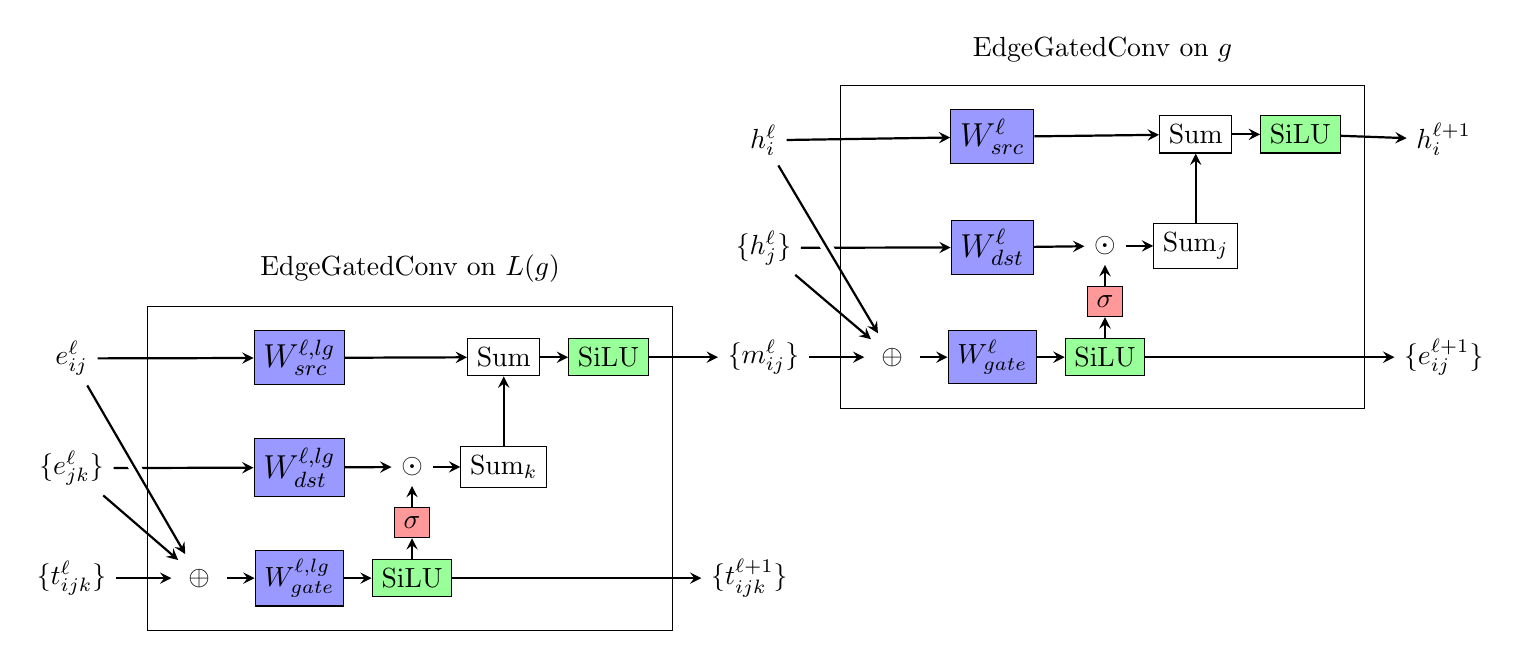
\begin{tikzpicture}

    %% \node (X1) {$h_{i}^{\ell}$};
    %% \node[below=2em of X1] (Xj) {$\{h_{j}^{\ell}\}$};
    %% \node[below=2em of Xj] (Eij) {$e_{ij}^{\ell}$};
    \node (Eij) {$e_{ij}^{\ell}$};
    \node[below=2em of Eij] (Ejk) {$\{e_{jk}^{\ell}\}$};
    \node[below=2em of Ejk] (Tijk) {$\{t_{ijk}^{\ell}\}$};

    %% line graph section

    %% \node[rectangle, right=1.2em of outj] (ink) {$\{e_{jk}^{\ell+\frac{1}{2}}\}$};
    %% \node[rectangle, above=1.75em of ink] (inj) {$e_{ij}^{\ell+\frac{1}{2}}$};

    %% \draw[-stealth, thick, opacity=0.4] (outj) -- (inj);
    %% \draw[-stealth, thick, opacity=0.4] (outj) -- (ink);

    \node[circle, right=2em of Tijk] (attnl) {$\oplus$};

    \node[rectangle, draw, right=1em of attnl, fill=white!60!blue] (Wgl) {$W_{gate}^{\ell,lg}$};
    \node[rectangle, draw, right=1em of Wgl, fill=white!60!green] (actgl) {SiLU};

    \node[rectangle, draw, above=1.9em of Wgl, fill=white!60!blue] (Wjl) {\large $W_{dst}^{\ell,lg}$};
    \node[rectangle, draw, above=1.9em of Wjl, fill=white!60!blue] (Wil) {\large $W_{src}^{\ell,lg}$};

    \draw[-stealth, thick] (Eij) -- (Wil);
    \draw[-stealth, thick] (Ejk) -- (Wjl);

    \draw[-stealth, line width=1.5mm, white] (Eij) -- (attnl);
    \draw[-stealth, thick] (Eij) -- (attnl);
    \draw[-stealth, thick] (Ejk) -- (attnl);
    \draw[-stealth, thick] (Tijk) -- (attnl);
    \draw[-stealth, thick] (attnl) -- (Wgl);
    \draw[-stealth, thick] (Wgl) -- (actgl);

    \node[rectangle, draw, above=0.75em of actgl, fill=white!60!red] (sigmoidl) {$\sigma$};
    \node[rectangle, above=0.75em of sigmoidl] (dotl) {$\odot$};

    \draw[-stealth, thick] (actgl) -- (sigmoidl);
    \draw[-stealth, thick] (Wjl) -- (dotl);
    \draw[-stealth, thick] (sigmoidl) -- (dotl);

    \node[rectangle, draw, right=1em of dotl] (aggregatel) {Sum$_k$};
    \draw[-stealth, thick] (dotl) -- (aggregatel);

    \node[rectangle, draw, above=2.5em of aggregatel] (combinel) {Sum};
    \draw[-stealth, thick] (aggregatel) -- (combinel);
    \draw[-stealth, thick] (Wil) -- (combinel);

    \node[rectangle, draw, right=1em of combinel, fill=white!60!green] (actl) {SiLU};
    \node[rectangle, right=2.5em of actl] (outil) {$\{m_{ij}^{\ell}\}$};
    \node[rectangle, right=9em of actgl] (outjl) {$\{t_{ijk}^{\ell+1}\}$};
    \draw[-stealth, thick] (combinel) -- (actl);
    \draw[-stealth, thick] (actl) -- (outil);
    \draw[-stealth, thick] (actgl) -- (outjl);

    \node[rectangle,draw, fit=(Wil) (attnl) (Wgl) (actl),inner sep=3mm](lglayer) {};


    %% % crystal graph section
    \node[above=2em of outil] (Xj) {$\{h_{j}^{\ell}\}$};
    \node [above=2em of Xj](X1) {$h_{i}^{\ell}$};

    \node[circle, right=2em of outil] (attn) {$\oplus$};
    \node[rectangle, draw, right=1em of attn, fill=white!60!blue] (Wg) {$W_{gate}^\ell$};
    \node[rectangle, draw, right=1em of Wg, fill=white!60!green] (actg) {SiLU};

    \node[rectangle, draw, above=2em of Wg, fill=white!60!blue] (Wj) {\large $W_{dst}^\ell$};
    \node[rectangle, draw, above=2em of Wj, fill=white!60!blue] (Wi) {\large $W_{src}^\ell$};

    \draw[-stealth, thick] (X1) -- (Wi);
    \draw[-stealth, thick] (Xj) -- (Wj);

    \draw[-stealth, line width=1.5mm, white] (X1) -- (attn);
    \draw[-stealth, thick] (X1) -- (attn);
    \draw[-stealth, thick] (Xj) -- (attn);
    \draw[-stealth, thick] (outil) -- (attn);
    \draw[-stealth, thick] (attn) -- (Wg);
    \draw[-stealth, thick] (Wg) -- (actg);

    \node[rectangle, draw, above=0.75em of actg, fill=white!60!red] (sigmoid) {$\sigma$};
    % \node[rectangle, right=4.5em of Wj] (dot) {$\odot$};
    \node[rectangle, above=0.75em of sigmoid] (dot) {$\odot$};

    \draw[-stealth, thick] (actg) -- (sigmoid);
    \draw[-stealth, thick] (Wj) -- (dot);
    \draw[-stealth, thick] (sigmoid) -- (dot);

    \node[rectangle, draw, right=1em of dot] (aggregate) {Sum$_j$};

    \draw[-stealth, thick] (dot) -- (aggregate);

    \node[rectangle, draw, above=2.5em of aggregate] (combine) {Sum};
    \draw[-stealth, thick] (aggregate) -- (combine);
    \draw[-stealth, thick] (Wi) -- (combine);

    \node[rectangle, draw, right=1em of combine, fill=white!60!green] (act) {SiLU};
    \node[rectangle, right=9em of actg] (outj) {$\{e_{ij}^{\ell+1}\}$};
    \node[rectangle, above=5.9em of outj] (outi) {$h_i^{\ell+1}$};
    \draw[-stealth, thick] (combine) -- (act);
    \draw[-stealth, thick] (act) -- (outi);
    \draw[-stealth, thick] (actg) -- (outj);

    \node[rectangle,draw, fit=(Wi) (attn) (Wg) (act),inner sep=3mm](layer) {};

    \node[rectangle, above=0.5em of layer] (text) {EdgeGatedConv on $g$};
    \node[rectangle, above=0.5em of lglayer] (lgtext) {EdgeGatedConv on $L(g)$};




\end{tikzpicture}
\end{document}
